\documentclass[journal]{./IEEE/IEEEtran}
\usepackage{cite,graphicx,float}

\newcommand{\SPTITLE}{Algorithmic Approaches to Classic Strategy Games - A Comparative Analysis of Search Techniques}
\newcommand{\ADVISEEA}{Clarence Joshua T. Bernardino}
\newcommand{\ADVISEEB}{Elisha Julianne Claveria}

\newcommand{\BSCS}{Bachelor of Science in Computer Science}
\newcommand{\ICS}{Institute of Computer Science}
\newcommand{\UPLB}{University of the Philippines Los Ba\~{n}os}
\newcommand{\REMARK}{\thanks{Presented to the Faculty of the \ICS, \UPLB\
                             in partial fulfillment of the requirements
                             for the Degree of \BSCS}}
        
\markboth{CMSC 170 Introduction to Artificial Intelligence, \ICS}{}
\title{\SPTITLE}
\author{\ADVISEEA~and~\ADVISEEB%
\REMARK
}
% \pubid{\copyright~2006~ICS \UPLB} nag c-clip to nakakainis so comment out muna

%%%%%%%%%%%%%%%%%%%%%%%%%%%%%%%%%%%%%%%%%%%%%%%%%%%%%%%%%%%%%%%%%%%%%%%%%%

\begin{document}

% TITLE
\maketitle

% SECTION 1
\section{Introduction}
Classic games such as Tic-Tac-Toe and the 8-puzzle have long served as foundational models for problem-solving and cognitive development. While traditionally associated with human recreation, these games also provide a structured and well-defined domain for evaluating the efficacy of artificial intelligence search algorithms. This paper presents a formal analysis of these canonical problems, transposing them from a human context to a computational one. We implement and systematically evaluate four fundamental search strategies, Breadth-First Search (BFS), Depth-First Search (DFS), the A* algorithm, and the Minimax decision rule, to solve and play these games autonomously. The objective of this study is to compare the performance of these algorithms in terms of completeness, optimality, time complexity, and space complexity, illustrating the practical trade-offs in automated problem-solving.

\subsection{Algorithmic comparison of BFS, DFS, A*, minimax}
What is your understanding of the algorithms based on the three exercises?

\subsection{Breadth-First Search (BFS) and Depth-First Search (DFS)}
The search algorithms can be characterized by their distinct exploration strategies. BFS and DFS are categorized as "blind" search strategies, as they traverse the board systematically without utilizing any information other than depth to guide the search toward a goal.\cite{geeksforgeeks-Uninformed-Search-Algorithms-in-AI}

\subsection{A* Search}
In contrast, the A algorithm* is an informed search method that uses a heuristic function, h(n), to guide its exploration toward the goal. It prioritizes nodes by minimizing the total estimated cost, f(n) = g(n) + h(n), where g(n) is the known path cost. This strategy is proven to be both complete and optimal, provided the heuristic never over-estimates the path-cost from any given node.\cite{geeksforgeeks-A-star-Search-Algorithm}

\subsection{Minimax Search}
For adversarial environments, the Minimax algorithm offers a strategic framework that is guaranteed to produce optimal play against a rational opponent. The algorithm recursively evaluates a game tree by propagating static evaluation scores from terminal states back to the root. A value of +1 is assigned to a win for the maximizing player, and -1 for a win for the minimizing player. The maximizing player selects moves that lead to the highest-valued states, while the minimizing player chooses moves leading to the lowest-valued states. Consequently, an agent implementing Minimax is assured of selecting the most advantageous move available in any given state.\cite{geeksforgeeks-Adversarial-Search-Algorithms-in-Artificial-Intelligence-(AI)}

% SECTION 2
\section{Methods}
The implementation of the 8-puzzle employed the DFS, BFS, and A* algorithms. By representing board states as strings and utilizing hashing via Python sets, the design ensured an efficient solution. The Tic-Tac-Toe game, on the other hand, utilized a class-based implementation to encapsulate the board state, thereby eliminating the redundancy of passing state through function parameters. This object-oriented approach provided a structured framework for implementing the Minimax algorithm, which recursively evaluates potential moves to determine the optimal strategy.

% formatting sources - 
% https://www.overleaf.com/learn/latex/Lists
% https://tex.stackexchange.com/questions/48632/underscores-in-words-text
\subsection{8-puzzle Implementation (Full Code in Appendix)}
\begin{itemize}
  \item \texttt{find\_gap(board)} – Locates the index of the blank tile ('0') within the string-encoded board state.

  \item \texttt{finished\_state(board)} – Returns True if the current board state matches the goal configuration ('123456780').

  \item \texttt{get\_possible\_moves(board)} – Determines all valid actions ('w', 'a', 'x', 'd') for the blank tile based on its grid position.

  \item \texttt{apply\_move(board, direction)} – Generates and returns a new board state by swapping the blank tile with an adjacent tile in the given direction.
\end{itemize}

\begin{itemize}
  \item \texttt{solve\_bfs(initial\_state)} – Explores the state space using a FIFO queue, guaranteeing a shortest-path solution.

  \begin{figure}[H]
    \centering
    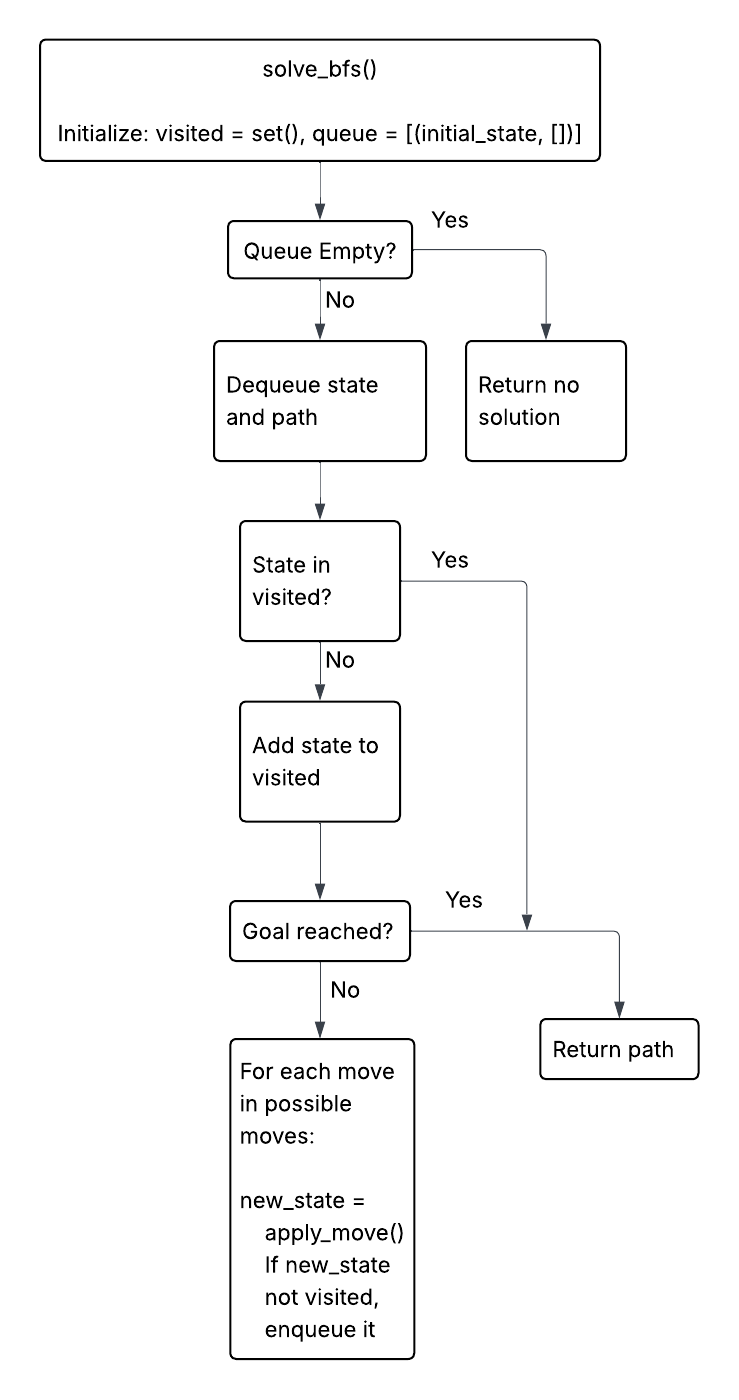
\includegraphics[width=0.6\linewidth]{pictures-Clarence/bfs flowchart.png}
    \caption{BFS Flowchart Diagram}
    \label{fig:bfs}
\end{figure}

  \item \texttt{solve\_dfs(initial\_state)} – Explores the state space using a LIFO stack, prioritizing depth-first expansion.
  
  \begin{figure}[H]
    \centering
    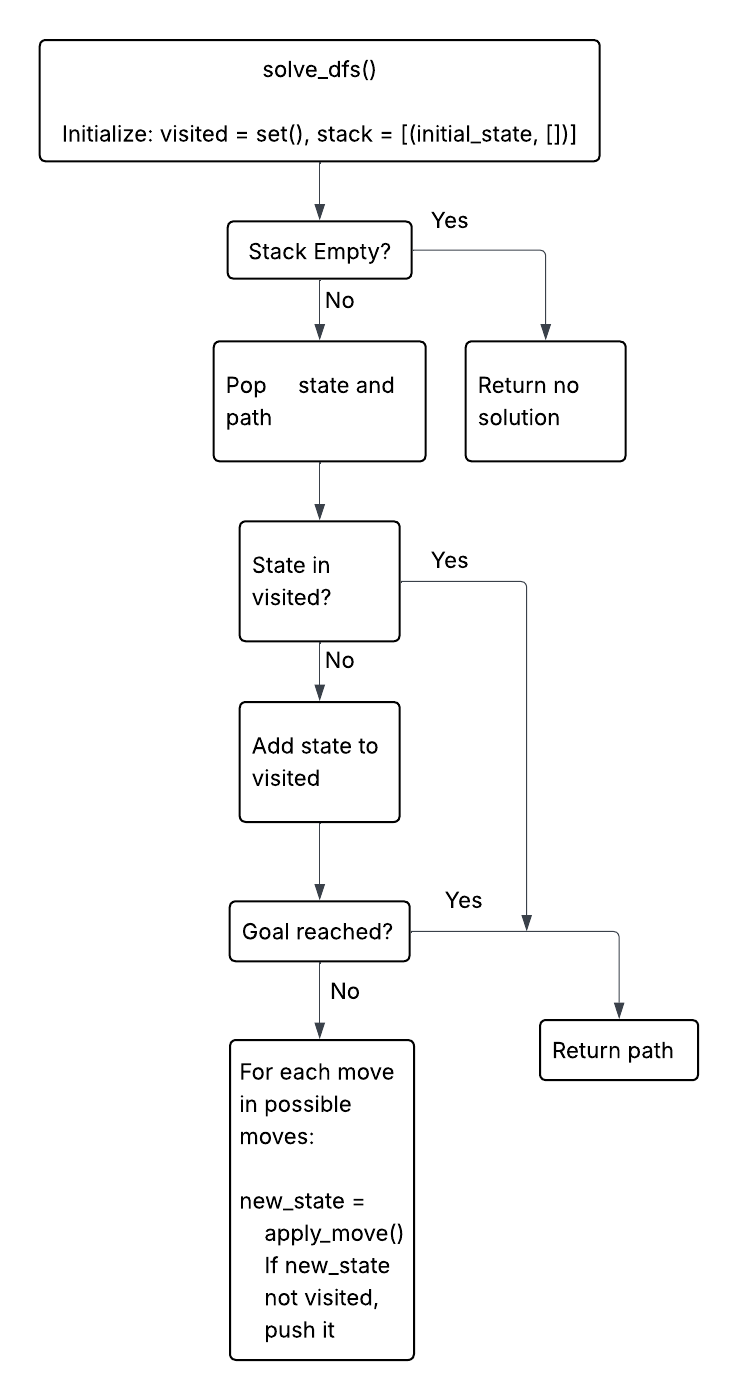
\includegraphics[width=0.6\linewidth]{pictures-Clarence/dfs flowchart.png}
    \caption{DFS Flowchart Diagram}
    \label{fig:dfs}
  \end{figure}

  \item \texttt{heuristic\_manhattan(board)} – Computes the sum of the Manhattan distances of each tile from its goal position.

  \item \texttt{solve\_astar(initial\_state, heuristic)} – Explores states by prioritizing the lowest estimated total cost (F = path cost (G) + heuristic (H)).

  \begin{figure}[H]
    \centering
    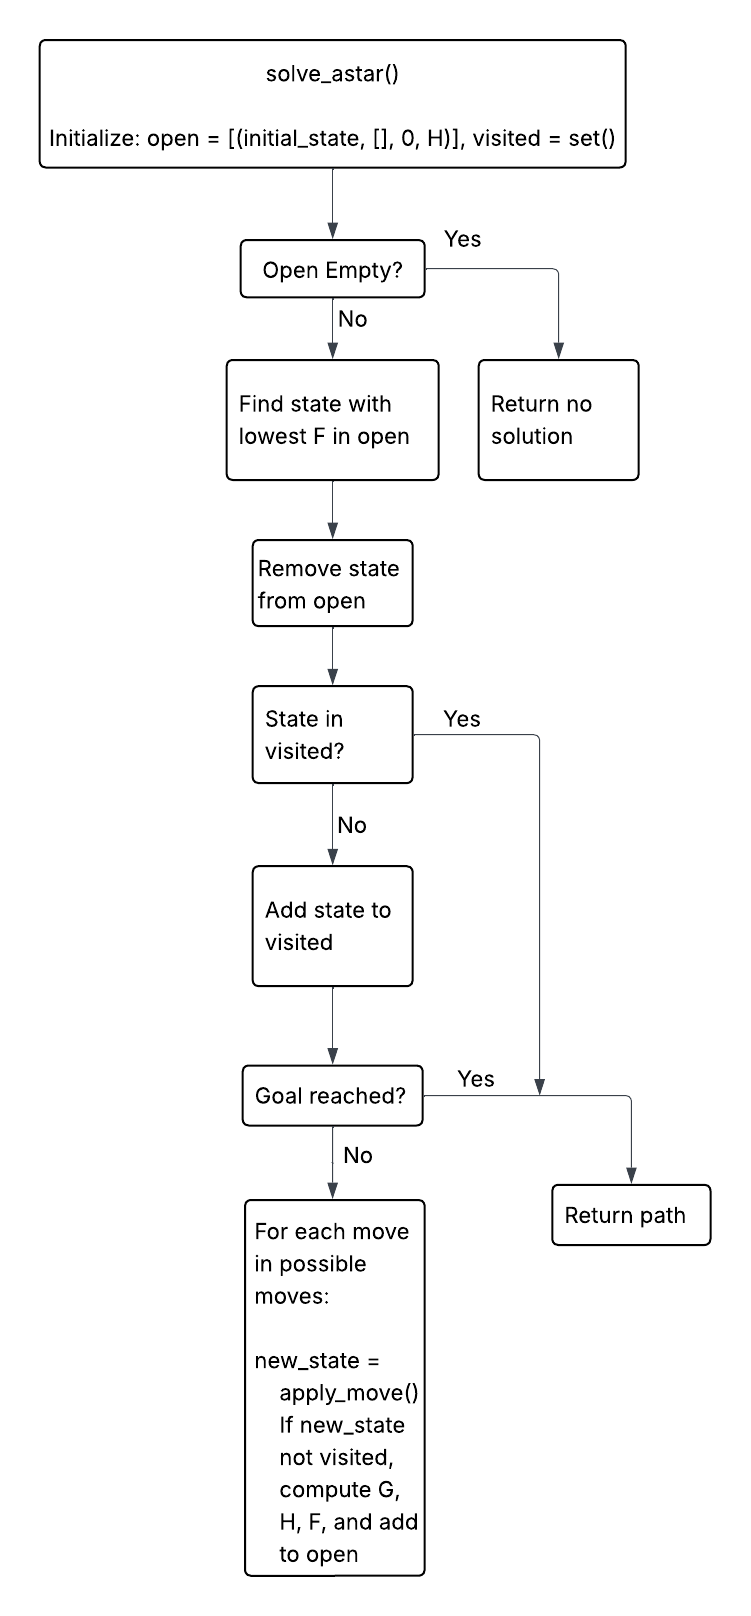
\includegraphics[width=0.6\linewidth]{pictures-Clarence/astar flowchart.png}
    \caption{Astar Flowchart Diagram}
    \label{fig:placeholder}
  \end{figure}

\end{itemize}

\subsection{Tic-Tac-Toe Implementation(Full Code in Appendix)}

\begin{itemize}
  \item \texttt{BoardState Class} – Represents the game state with a 3x3 grid, tracks moves, and manages board operations.

  \item \texttt{apply\_move(row, col, is\_x)} – Places an 'X' or 'O' on the board at the specified position.

  \item \texttt{undo\_move(row, col)} – Reverts a move by clearing the specified position, essential for state exploration in Minimax.

  \item \texttt{get\_winner()} – Evaluates the board and returns the symbol of the winning player or None if no winner.

  \item \texttt{minmax()} – A recursive minimax algorithm that evaluates all possible moves to return a score for the current board state (-1, 0, 1).
\end{itemize}

\begin{figure}[H]
    \centering
    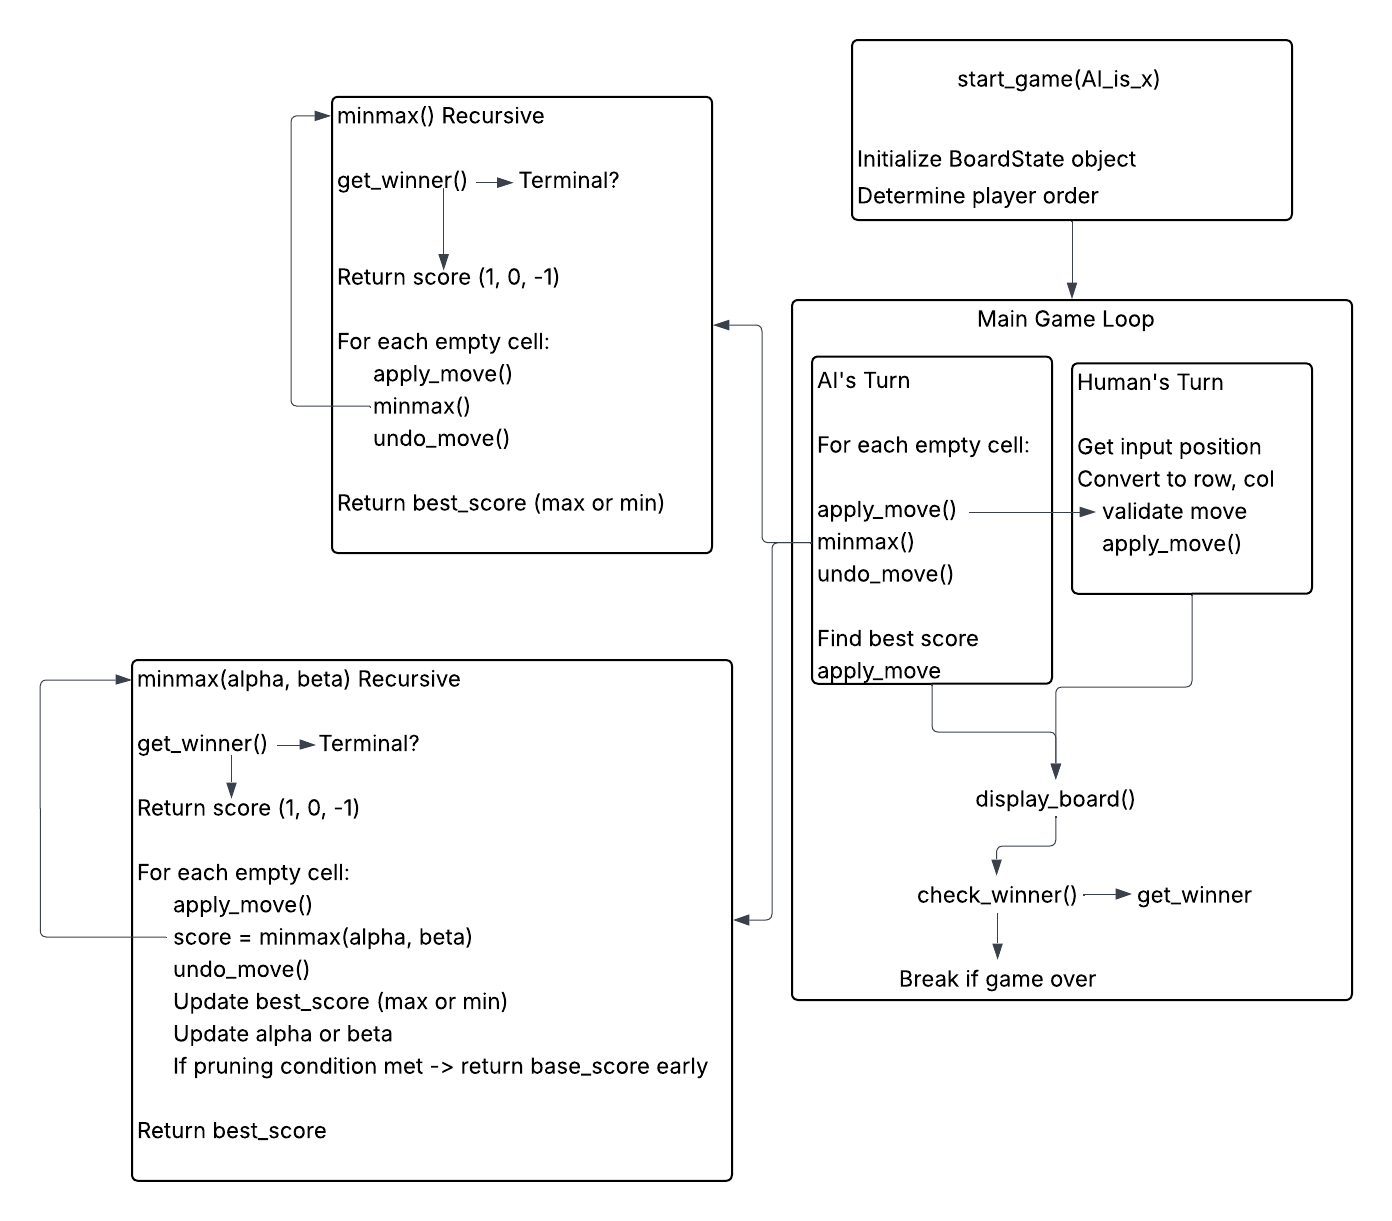
\includegraphics[width=0.6\linewidth]{pictures-Clarence/minmax flowchart.png}
    \caption{Minmax Flowchart Diagram}
    \label{fig:placeholder}
\end{figure}

\subsubsection{Choice of data structure, per algorithm, per exercise; and}
\subsubsection{What are the differences between each one’s implementation ?}
For the 8-puzzle solver, the uninformed search algorithms utilized distinct frontier management structures. Breadth-First Search employed a queue to guarantee that the shallowest, least-cost nodes were expanded first ensuring the shortest path at the cost of memory space. In contrast, Depth-First Search utilized a stack, prioritizing the deepest nodes in the current branch, which trades speed for reduced memory requirement per branch. The A* algorithm implemented the logic of a priority queue by maintaining an open list ordered by the sum F = G + H, where G is the path cost and H is the heuristic estimate. The node with the lowest F-cost was selected for expansion each iteration, guiding the search toward the goal.

For the adversarial Tic-Tac-Toe environment, the Minimax algorithm didn't use an external data structure for the frontier. Instead, its effectiveness derives from recursive state space exploration coupled with backtracking. The algorithm implicitly builds a game tree, leveraging the call stack to evaluate moves recursively. It employs a depth-first traversal to mark states with value -1 or 1 from terminal states back to the root, enabling the machine to select moves that maximize its advantage.
% SECTION 3
\section{Results}
The quick brown fox jumps over the lazy dog. The quick brown fox jumps over
the lazy dog. The quick brown fox jumps over the lazy dog. The quick brown
fox jumps over the lazy dog.

\subsection{Performance Evaluation}
The quick brown fox jumps over the lazy dog. The quick brown fox jumps over
the lazy dog. The quick brown fox jumps over the lazy dog. The quick brown
fox jumps over the lazy dog.

% SECTION 4
\section{Conclusion}
The quick brown fox jumps over the lazy dog. The quick brown fox jumps over
the lazy dog. The quick brown fox jumps over the lazy dog. The quick brown
fox jumps over the lazy dog.

\subsection{Real-world Application}
\subsubsection{... of the AI algorithms}
\subsubsection{What did you learn or realize about “How AI works?”?}

\subsection{Future improvements}
\subsubsection{... of the AI algorithms}
\subsubsection{What did you learn or realize about “How AI should be used responsibly?”?}

\subsection{Challenges}
\subsubsection{... of the AI algorithms}
\subsubsection{What did you learn or realize about “How AI is affecting society?”?}

% SECTION 5
\section{Responsible Use of AI}

\subsubsection{How much AI did you use? }
\subsubsection{Justification for responsible use}

% APPENDICES
\appendices

\section{Additional Code Snippets}
The quick brown fox jumps over the lazy dog. The quick brown fox jumps over
the lazy dog. The quick brown fox jumps over the lazy dog. The quick brown
fox jumps over the lazy dog.

% BIBLIOGRAPHY
\bibliographystyle{IEEE/IEEEtran}
\bibliography{cs190-ieee}
% \nocite{*}

% BIOGRAPHY
\begin{biography}[{
\includegraphics{./yourPicture.eps}}]{Student M. Name}
Biography text here...
\end{biography}


\end{document}
 
